\documentclass[
	fontsize=10pt, % Base font size
	twoside=false, % Use different layouts for even and odd pages (in particular, if twoside=true, the margin column will be always on the outside)
	%open=any, % If twoside=true, uncomment this to force new chapters to start on any page, not only on right (odd) pages
	%chapterprefix=true, % Uncomment to use the word "Chapter" before chapter numbers everywhere they appear
	%chapterentrydots=true, % Uncomment to output dots from the chapter name to the page number in the table of contents
	numbers=noenddot, % Comment to output dots after chapter numbers; the most common values for this option are: enddot, noenddot and auto (see the KOMAScript documentation for an in-depth explanation)
	%draft=true, % If uncommented, rulers will be added in the header and footer
	%overfullrule=true, % If uncommented, overly long lines will be marked by a black box; useful for correcting spacing problems
]{kaohandt}

% Choose the language
\usepackage[english]{babel} % Load characters and hyphenation
\usepackage[english=british]{csquotes}	% English quotes

% Load the bibliography package
\usepackage{styles/kaobiblio}
\addbibresource{main.bib} % Bibliography file

% Load the package for hyperreferences
\usepackage{styles/kaorefs}

% Set the paths where to look for images
\usepackage{subcaption}
\graphicspath{{examples/report/img/}{img/}}

\begin{document}

\title{Operation T-REx}
\author[FM]{Federico Marotta}
\date{December 2019}
\maketitle

\setchapterstyle{kao}
\setchapterpreamble[u]{\margintoc}
\chapter{Introduction}

\section{The main ideas}

Many modern printed textbooks have adopted a layout with prominent 
margins where small figures, tables, remarks and just about everything 
else can be displayed. Arguably, this layout helps to organise the 
	discussion by separating the main text from the ancillary material, 
	which at the same time is very close to the point in the text where 
	it is referenced.

This text does not aim to be an apology of wide margins, for there are 
many better suited authors for this task; the purpose of all these words 
is just to fill the space so that the reader can see how a book written 
with the kaobook class looks like. Meanwhile, I shall also try to 
illustrate the features of the class.

The main ideas behind kaobook come from this 
\href{https://3d.bk.tudelft.nl/ken/en/2016/04/17/a-1.5-column-layout-in-latex.html}{blog 
	post}, and actually the name of the class is dedicated to the author 
of the post, Ken Arroyo Ohori, which has kindly allowed me to create a 
class based on his thesis. Therefore, if you want to know more reasons 
to prefer a 1.5-column layout for your books, be sure to read his blog 
post.

Another source of inspiration, as you may have noticed, is the 
\href{https://github.com/Tufte-LaTeX/tufte-latex}{Tufte-Latex Class}. 
The fact that the design is similar is due to the fact that it is very 
difficult to improve something wich is already so good. However, I like 
to think that this class is more flexible than Tufte-Latex. For 
instance, I have tried to use only standard packages and to implement as 
little as possible from scratch;\sidenote{This also means that 
understanding and contributing to the class development is made easier. 
Indeed, many things still need to be improved, so if you are interested, 
check out the repository on github!} therefore, it should be pretty easy 
to customise anything, provided that you read the documentation of the 
package that provides that feature.

In this book I shall illustrate the main features of the class and 
provide information about how to use and change things. Let us get 
started.

\section{What this class does}
\labsec{does}

The kaobook class focuses more about the document structure than about 
the style. Indeed, it is a well-known \LaTeX\xspace principle that 
structure and style should be separated as much as possible (see also 
\vrefsec{doesnot}). This means that this class will only provide 
commands, environments and in general, the opportunity to do things, 
which the user may or may not use. Actually, some stylistic matters are 
embedded in the class, but the user is able to customise them with ease.

The main features are the following:

\begin{description}
	\item[Page Layout] The text width is reduced to improve readability 
	and make space for the margins, where any sort of elements can be 
	displayed.
	\item[Chapter Headings] As opposed to Tufte-Latex, we provide a 
	variety of chapter headings among which to choose; examples will be 
	seen in later chapters.
	\item[Page Headers] They span the whole page, margins included, and, 
	in twoside mode, display alternatively the chapter and the section 
	name.\sidenote[-2mm][]{This is another departure from Tufte's 
	design.}
	\item[Matters] The commands \Command{frontmatter}, 
	\Command{mainmatter} and \Command{backmatter} have been redefined in 
	order to have automatically wide margins in the main matter, and 
	narrow margins in the front and back matters. However, the page 
	style can be changed at any moment, even in the middle of the 
	document.
	\item[Margin text] We provide commands \Command{sidenote} and 
	\Command{marginnote} to put text in the 
	margins.\sidenote[-2mm][]{Sidenotes (like this!) are numbered while 
	marginnotes are not}
	\item[Margin figs/tabs] A couple of useful environments is 
	\Environment{marginfigure} and \Environment{margintable}, which, not 
	surprisingly, allow you to put figures and tables in the margins 
	(\cfr \reffig{marginmonalisa}).
	\item[Margin toc] Finally, since we have wide margins, why don't add 
	a little table of contents in them? See \Command{margintoc} for 
	that.
	\item[Hyperref] \Package{hyperref} is loaded and by default we try 
	to add bookmarks in a sensible way; in particular, the bookmarks 
	levels are automatically reset at \Command{appendix} and 
	\Command{backmatter}. Moreover, we also provide a small package to 
	enhance hyperreferences to other parts of the text.
	\item[Bibliography] We want the reader to be able to know what has 
	been cited without having to go to the end of the document every 
	time, so citations go in the margins as well as at the end, as in 
	Tufte-Latex. Unlike that class, however, you are free to customise 
	the citations as you wish.
\end{description}

\begin{marginfigure}[-5.5cm]
	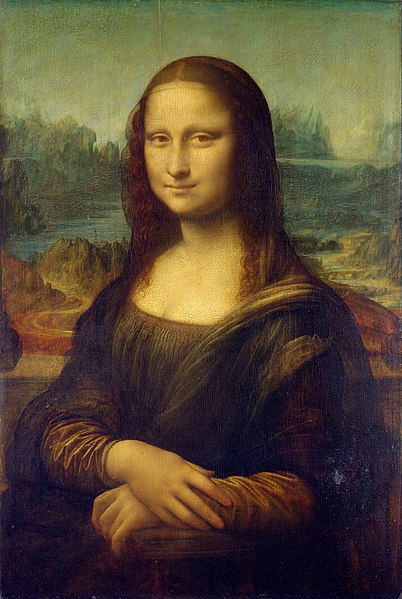
\includegraphics{monalisa}
	\caption[The Mona Lisa]{The Mona Lisa.\\ 
	\url{https://commons.wikimedia.org/wiki/File:Mona_Lisa,_by_Leonardo_da_Vinci,_from_C2RMF_retouched.jpg}}
	\labfig{marginmonalisa}
\end{marginfigure}

In addition, the class is based on \KOMAScript's \Class{scrbook}, 
therefore it inherits all the goodies of that.

\section{What this class does not}
\labsec{doesnot}

As anticipated, further customisation of the book is left to the user. 
Indeed, every book may have sidenotes, margin figures and so on, but 
each book will have its own fonts, toc style, special environments and 
so on. For this reason, in addition to the class, we provide only 
sensible defaults, but if these features are not nedded, they can be 
left out. These special packages are located in the \Path{style} 
directory, which is organised as follows:

\begin{description}
	\item[style.sty] This package contains the specifications of page 
	layout, headers and footers, chapter headings, and the fonts used 
	throughout the document.
	\item[packages.sty] Loads additional packages to decorate the 
	writing with special contents (for instance, the \Package{listing} 
	package is loaded here as it is not required in every book). There 
	are also defined some useful commands to print the same words always 
	in the same way, \eg latin words in italics or \Package{packages} in 
	verbatim.
	\item[references.sty] Some useful commands to manage labeling and 
	referencing, again to ensure that the same elements are referenced 
	always in a consistent way.
	\item[environments.sty] Provides special environments, like boxes. 
	Both simple and complex environments are available; by complex we 
	mean that they are endowed with a counter, floating and can be put 
	in a special table of contents.\sidenote[-2mm][]{See 
	\vrefch{mathematics} for some examples.}
	\item[theorems.sty] The style of mathematical environments. 
	Acutally, there are two such packages: one is for plain theorems, 
	\ie the theorems are printed in plain text; the other uses 
	\Package{mdframed} to draw a box around theorems. You can plug the 
	most appropriate style into its document.
\end{description}

\marginnote[2mm]{The audacious users might feel tempted to edit some of 
these packages. I'd be immensely happy if they sent me examples of what 
they have been able to do!}

In the rest of the book, I shall assume that the reader is not a novice 
in the use of \LaTeX, and refer to the documentation of the packages 
used in this class for things that are already explained there. 
Moreover, I assume that the reader is willing to make minor edits to the 
provided packages for styles, environments and commands, if he or she 
does not like the default settings.

\section{Data}
\labsec{data}

The Genotype-Tissue Expression (GTEx) project \sidecite{Lonsdale2013a} 
aims to characterise gene expression and regulation for 54 human healthy 
tissues across nearly 1000 people. While the results of the analyses are 
open-access, in order to gain access to the raw data about the DNA and 
the gene expression of the individuals, it is necessary to go through a 
long bureaucratic procedure.

Another source of data was the Ensembl project (release 75), 
\sidecite[-5\baselineskip-2mm]{Zerbino2018} which was used to obtain the 
coordinates of the regulatory regions for each gene. Regulatory regions 
are particular positions around a gene where transcription factors can 
bind; from there, these transcription factors exert a control on gene 
expression.\sidenote{In this project, I considered 141 genes of a 
particular type of blood cells, for 95 individuals. Each gene is 
associated to about 10 regulatory regions on average.} Each 
transcription factor recognises a specific sequence of DNA, therefore it 
is possible to compute the affinity of a factor for a given region. The 
total binding affinity (TBA) 
\sidecite[-10\baselineskip-2.8mm+1pt]{Molineris2011a} is one of the 
possible affinity measures.

Gene expression in GTEx was measured with a technique called RNA-seq, 
which, through the sequencing of the RNA, allows us to count how many 
molecules there are and to associate them to the gene where they come 
from. The raw expression files contain, for each gene and each 
individual, the RPKM, \sidecite[-13\baselineskip-1mm]{Mortazavi2008} 
that is, the number of sequencing reads normalised by the length of the 
gene and by the total number of reads.

The gene expression was preprocesed as recommended by the Stephen's 
Lab.\sidenote{\url{http://stephenslab.github.io/gtex-eqtls/analysis/20170515\_RNASeq\_Analysis.html}} 
In summary, I applied a quantile normalisation to make sure that the 
distribution of our response variable was normal, and then I obtained 
the residuals of a linear model \\
$Y~\sim~SEX+PEER\_FA+POPULATION+PLATFORM$, so as to disregard the 
effects of these covariates on the expression. The final result can be 
seen in \reffig{distrexpr}.

\begin{figure}[b]
  \centering
  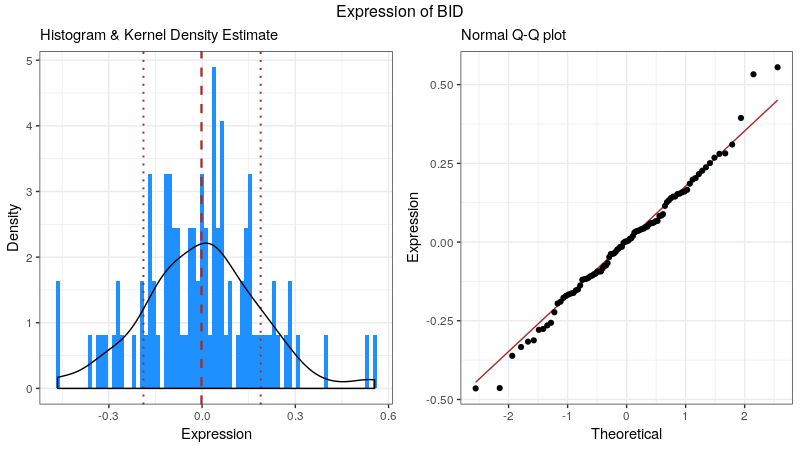
\includegraphics[height=5.2cm,width=.9\textwidth,keepaspectratio=false]{bid_expr}
  \caption{Histogram and normal Q\babelhyphen{nobreak}Q plot of the 
expression of a randomly selected gene called BID. In the histogram, the 
brown dashed line indicates the mean, while the dotted lines indicate 
plus and minus one standard deviation. In the Q\babelhyphen{nobreak}Q 
plot, each point represents an individual.}
  \labfig{distrexpr}
\end{figure}

\begin{figure}[t]
  \centering
  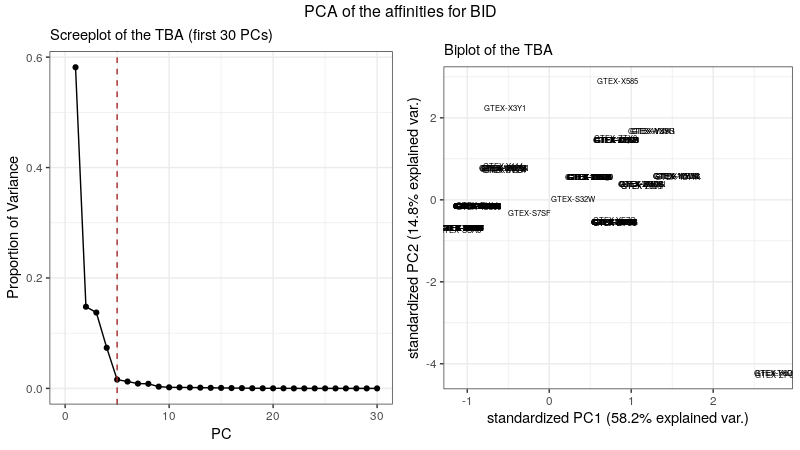
\includegraphics[height=5.2cm,width=.9\textwidth,keepaspectratio=false]{bid_tba}
  \caption{Scree plot and biplot of the \textasciitilde800 affinities for the gene 
BID. In the biplot, each label corresponds to an individual.}
  \labfig{pcatba}
\end{figure}

The genotypes were also obtained with a sequencing technique and were 
provided in VCF format. \sidecite[-22\baselineskip+.4mm]{Danecek2011} I 
used a software called 
\nohyphens{VCF\textunderscore\nobreak\hspace{0pt}rider}\sidenote{\url{https://github.com/vodkatad/vcf\_rider}} 
to compute the total binding affinity of each transcription factor for 
each regulatory region associated to a gene (the total number of 
transcription factors is about 800). \reffig{pcatba} reports the PCA of 
the TBA for the gene BID.

\section{Results}
\labsec{results}

\subsection{Nested Cross-Validation Package}

All the similar published works use a 5-fold cross-validation to 
evaluate their models. However, since there are also some parameters to 
tune, they rely on a (computationally expensive) netsed cross-validation 
in order not to overestimate the predictive power. Since I needed to run 
several different models for each of the 140 genes, each with its own 
parameters, I decided to write an R 
package\sidenote[][-2.3cm]{\url{https://github.com/fmarotta/cvtools}} to 
perform the nested cross-validation with a heuristic algorithm that does 
not try all the possible values for the parameters, but rather, 
independently for each parameter, it starts at one value and explores 
the adjacent ones; then, it moves in the direction where the error 
decreases
(\reffig{cv}).

\begin{marginfigure}[-3.4cm]
  \centering
  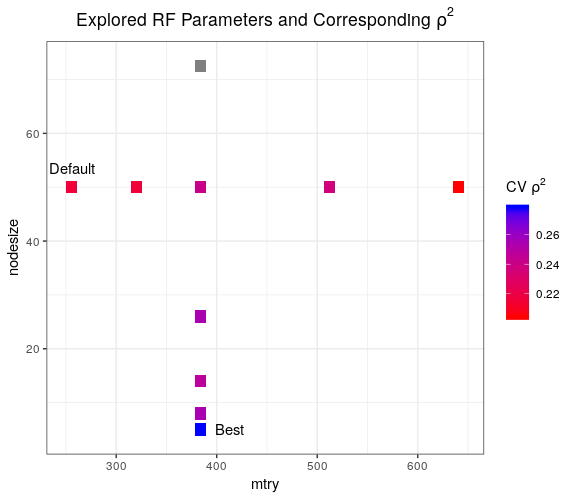
\includegraphics{cv}
  \caption{First, the mtry is tuned while the nodesize is kept fixed; 
the algorithm started at the default value of 256, then it moved up in 
the range as long as the error decreased, and finally it came back to 
explore the values in between. Next, the nodesize was tuned in a similar 
fashion.}
  \labfig{cv}
\end{marginfigure}

This package requires the user to write a function which takes 
predefined arguments and returns a predefined output, but except for 
that, it can be used with any regression model. I evaluated the 
performances of ridge, BART, random forest, and PCR. 
\sidecite[-12.9cm]{James2013a,Hastie2009}

\subsection{Model Performance}

The measure of performance is not the MSE nor the $R^2$, but rather the 
square of the correlation between true and predicted expression 
($\rho^2$); indeed, we do not want to penalise errors on single 
individuals, but we are interested in the general trend of expression. I 
decided to compare my results with those of TIGAR, \cite{Nagpal2019} 
which is currently most recent paper on this topic.

\begin{table}[b]
  \caption{Mean $\rho^2$ across 141 genes. The t-test was always 
performed with respect to TIGAR.}
  \labtab{comp}
  \begin{tabular}{lcc}
  \textbf{Model} & \textbf{Mean} \boldmath$\rho^2$ & \textbf{t-test pval} \\
  \midrule
  TIGAR & 0.067 & NA\\
  Ridge & 0.076 & 0.025\\
  BART & 0.074 & 0.121\\
  Ranger & 0.069 & 0.398\\
  PCR & 0.064 & 0.737\\
  \end{tabular}
\end{table}

Even if it captures only the linear relationships, ridge gave the best 
predictive performance (\reffig{rho2distr}), probably because in this 
context where $p >> n$, it is a good compromise between bias, variance 
and overfitting. According to a t-test, the $\rho^2$ achieved by ridge 
with the TBA values are even higher than those obtained by TIGAR 
(\reftab{comp}).

\begin{marginfigure}[-2cm]
  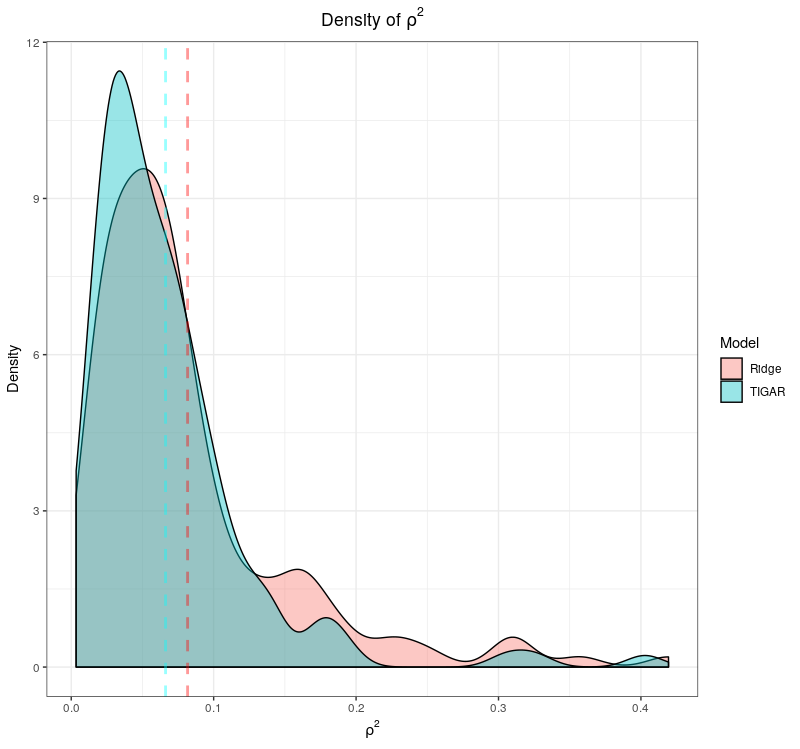
\includegraphics{rho2distr}
  \caption{Density plot of the $\rho^2$ achieved by T-REx (Ridge) and 
TIGAR. The dotted lines denotes the means of the 
distributions.}
  \labfig{rho2distr}
\end{marginfigure}

The performance of BART was not so different, despite the method being 
completely different. However, an important advantage of BART with 
respect to ridge is its ability to provide importance measures, allowing 
us to find which transcription factors are important for each gene. 
Additionally, BART captures the interactions between transcription 
factors.

The other methods, random forest and principal component regression, 
were much less powerful.

\subsection{Considering the Expression of the Transcription Factor}

As high as its affinity for the DNA may be, if the transcription factor 
is present only in tiny amounts it will not bind many regulatory 
regions. For this reason, we tried to enhance our predictors with 
information from the expression of the transcription factors.

\marginnote{%
The Hill equation models the rate of expression of a gene:
\begin{equation*}
  \theta = w \frac{L^n}{K^n + L^n} \approx w \left(\frac{L}{K}\right)^n.
\end{equation*}
Here, $L$ is the amount of transcription factor, $K$ is the dissociation 
constant (the inverse of the affinity), and $w$ is a constant. It is 
reasonable to suppose that if many transcription factors regulate a 
gene, the rate will be given by the following product, where we denoted 
$A = 1 / K$:
\begin{equation*}
  \theta = w_1 \left( L_1 A_1 \right)^{n_1} \cdots w_p \left( L_p A_p \right)^{n_p}.
\end{equation*}
Now, if we compute the log of the rate, we get a linear combination 
which in principle is a deterministic function, but in practice we can 
use this linear combination as the right-hand side of a model formula 
and let ridge estimate the coefficients:
\begin{align*}
  Y \sim \beta_0 &+ \beta_1 \left(\log L_1 + \log A_1\right) \\
                 &+ \cdots \\
                 &+ \beta_p \left(\log L_p + \log A_p\right).
\end{align*}
}

In the dataset, we have expression values for some 40.000 genes; of 
these, about 800 are transcriptional factors. In practice we removed 
those rows from the dataset, and summed the TBA and the expression of 
corresponding transcription factors. The new predictors gave a 
considerable improvement in the performance, and, perhaps surprsingly, 
ridge outclassed BART. In the adjacent margin note I describe the 
working hypothesis more in detail.

\begin{table}[H]
  \begin{tabular}{lr}
  \textbf{Model} & \textbf{Mean} \boldmath$\rho^2$ \\
  \midrule
  Ridge & 0.393\\
  BART & 0.268\\
  \end{tabular}
\end{table}


\section{Discussion}
\labsec{discussion}

Instead of finding a better model, in this project I tried to find 
better predictors. Using the affinities instead of the genotypes has 
several advantages:

\begin{itemize}
  \item The model is more interpretable (\eg we can say that as the 
affinity increases, the expression increases);
  \item The number of predictors decreases;
  \item The predictive power is higher;
\end{itemize}

Upon doing some biochemical considerations, it is possible to find even 
better predictors, although they violate the constraint of using only 
the DNA sequence to predict gene expression.

There are many ways to continue this work. One would be to construct an 
ensemble model that chooses, for each gene, the model that achieved the 
best prediction on a training set.

Another possibility is that of exploiting further the interpretability 
of this model, and use the trees produced by BART to make inferences 
about the regulatory network among genes.

Finally, one of the biggest limitations of these kind of models is that 
they consider each gene as independent of all the others. One possible 
way to use the information hidden among other genes is what I call the 
\enquote{bagging of the genes,} where the prediction for a new gene is 
given by the average of the prediction of a number of other models 
trained on different genes.

If we were able to accurately predict gene expression, the benefit would 
be twofold: first, it would be possible to predict which individuals are 
at risk of developing a disease, and consequently to prevent it; 
secondly, the biological mechanisms through which the illnesses arise 
would be elucidated, potentially leading to the discovery of new 
therapeutic targets. In conclusion, I hope that this project will give a 
contribution, albeit very small, in understanding the relationships 
between genome, expression and diseases.


\defbibnote{bibnote}{Here are the references in citation order.\par\bigskip} % Prepend this text to the bibliography
\renewcommand*{\bibfont}{\small}
\printbibliography[title=Bibliography]% , prenote=bibnote]

\end{document}
